\chapter{Design and implementation}
In this chapter the design and system architecture of the product will be presented. The reader will learn about how the different components of the product is put together, and how the design of the application was planned.

\section{System Architecture}
	The design was divided into several modules:
	\begin{itemize}
		\item{Bluetooth$\textsuperscript{\textregistered}$ connection between the Android and the Arduino}
		\item{Synchronization with the local SQLite database}
		\item{Android application view (the visible design)}
		\item{A service that contains the protocol for installing ``over the air''}
	\end{itemize}
	\vspace{0.2in}
	
	The system design was implemented such that further developing and extension should be as modular and easy as possible.
	Therefore it was designed as a plugin-like system where you easily can implement your own protocols against a desired device, e.g. Raspberry Pi. The application only supports the STK500 protocol and therefore only connections towards Arduino devices (and with some work other STK500 based devices).
	The design for the connection to other devices was done as shown in Figure~\ref{fig:btconnection}\\

	\begin{figure}[H]
	\centering
	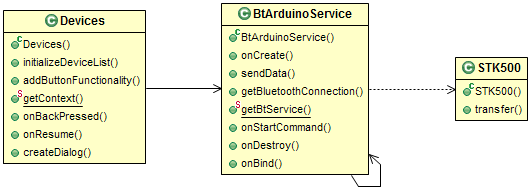
\includegraphics[width=130mm]{images/BTConnection.png}
	\caption{Bluetooth Connection between Android and Arduino stored in a service}
	\label{fig:btconnection}
	\end{figure}

	Devices.java is an Activity and can therefore be considered as a view in the application. To add a new service a few changes to Devices.java would have to be done. Another service and a protocol towards a desired device must be implemented, or support for multiple services. Since this project only considers connections between Android and Arduino, only the STK500 protocol was implemented.
	The overall design solution for multiple connections will be like in Figure~\ref{fig:otaarchitecture}\\
	\begin{figure}[H]
	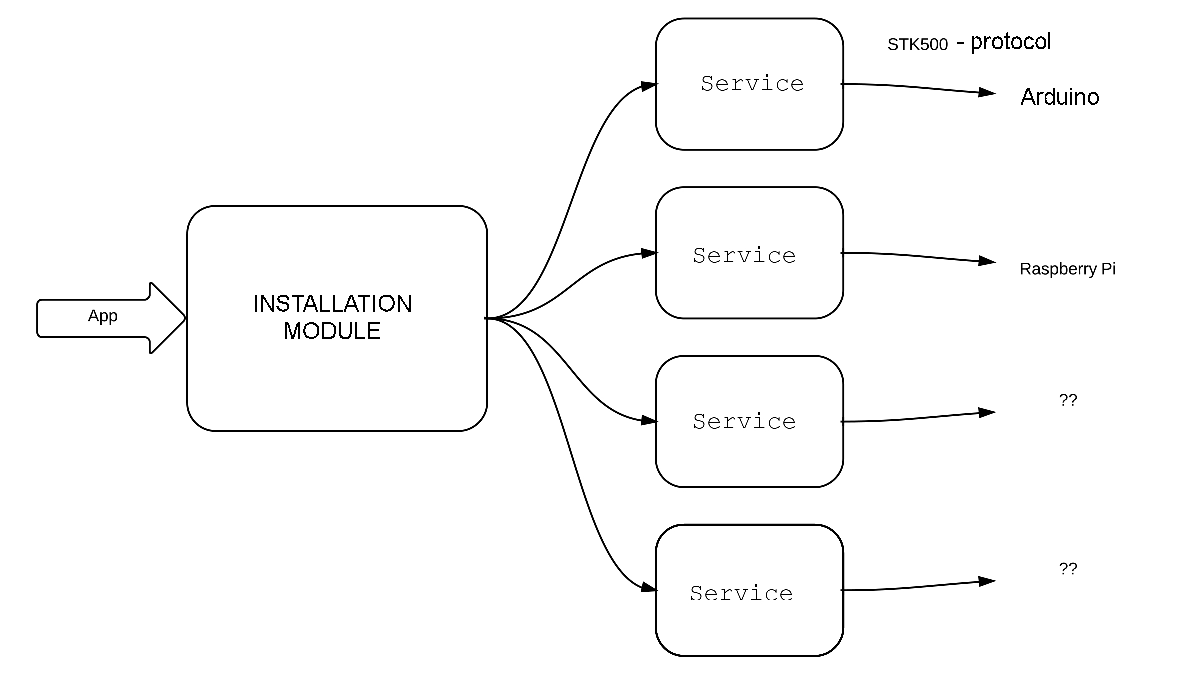
\includegraphics[scale=0.7]{figures/OTAArchitecture.pdf}
	\caption{Over The Air Architecture}
	\label{fig:otaarchitecture}
	\end{figure}

	The overall system architecture as shown in Figure~\ref{fig:systemarchitecture} illustrates the core components of the system and the relationship between these components. The \textit{Market Application} is the center of the application and is where most the GUI and functionality to the user is taking place. \textit{Device List} is the list of devices that the user can choose from and connect to. It is also here the \textit{Add Device} functionality is, where the user can connect to a device on an alternative way (QR or MAC-address).\\

	The \textit{Service} holds and manages the bluetooth connection (\textit{BluetoothConnection}) and is taking care of the protocol for installing apps on the microcontroller. \\

	The \textit{Memory card} is the memory card on the mobile phone where the database is stored (locally). SQLite was used for database engine because it is common and easy to implement in Android.\\

	\textit{DatabaseHandler} is a class for taking care of the SQL transactions and is the access point for communication with the database. A helper class called \textit{Save} is used for easy access to the \textit{DatabaseHandler}.
	When the application communicates with the Save module, the database communicates with the DatabaseHandler.
	\textit{Save} was created because it can be initialized and created everywhere in the application (in optional java classes) and makes sure its only one instance of the \textit{DatabaseHandler}.



	\begin{figure}[H]
	\centering
	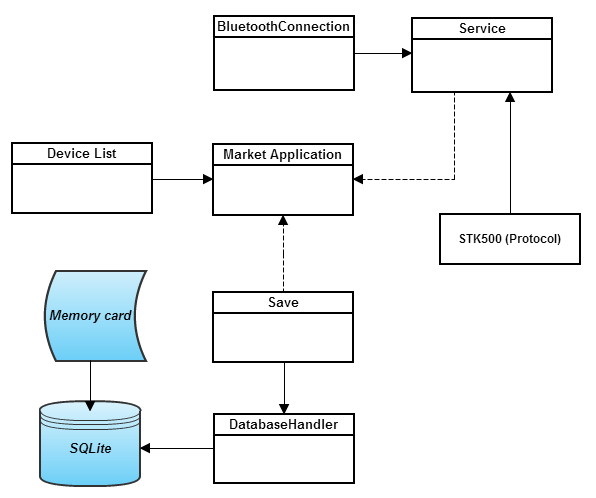
\includegraphics[scale=0.8]{images/System_architecture.png}
	\caption(System Architecture){This shows the overall system architecture with the most important components}
	\label{fig:systemarchitecture}
	\caption{The design for the connection of Bluetoot devices.}
	\label{BTConnection}
	\end{figure}


\section{Design of Android application}
One of the purposes of the Android application was to ease the process of installing PUIs on an Arduino for non-technical users. As described in section \ref{non-functional}, one of the requirements for the project was that people of all ages are supposed to understand how to use the application. This requirement put pressure on the design, as one have to make sure everyone are able to understand the different functions of the application. \\
\newline
Before the programming of the Android application was started, a complete design guide were created. In this section the complete design of the application is presented. This guide was made for primarily two reasons:
\begin{itemize}
	\item{Presentation for the customer:} With a complete design guide it was possible to present the user interface of the application to the customer before it was programmed. This allowed for input from the customer at an early stage, when it was easier to change the design.
	\item{Avoid confusion:} A design guide reduces the amount of confusion and discussion regarding the appearance of the user interface. When the looks of the user interface was settled before the programming had started, there was less need to discuss this along the way.
\end{itemize}

\subsection{Design guide}
Following is the complete design guide of the Android application. Minor changes were made to some of the screens. In these cases it is commented below the picture. The design of the preferences screen is not shown, as it was unnecessary to design this screen since it is a standard for Android applications.

\paragraph{Screen 1a - Device list}
Screen that shows the list of available Arduino devices. In the final design the list of devices fills the whole screen, and the buttons and description text have switched places. When a device is clicked, a progress bar appears and stays on the screen until a valid Bluetooth$\textsuperscript{\textregistered}$ connection with the chosen device is made.

\begin{figure}[H]
	\centering
		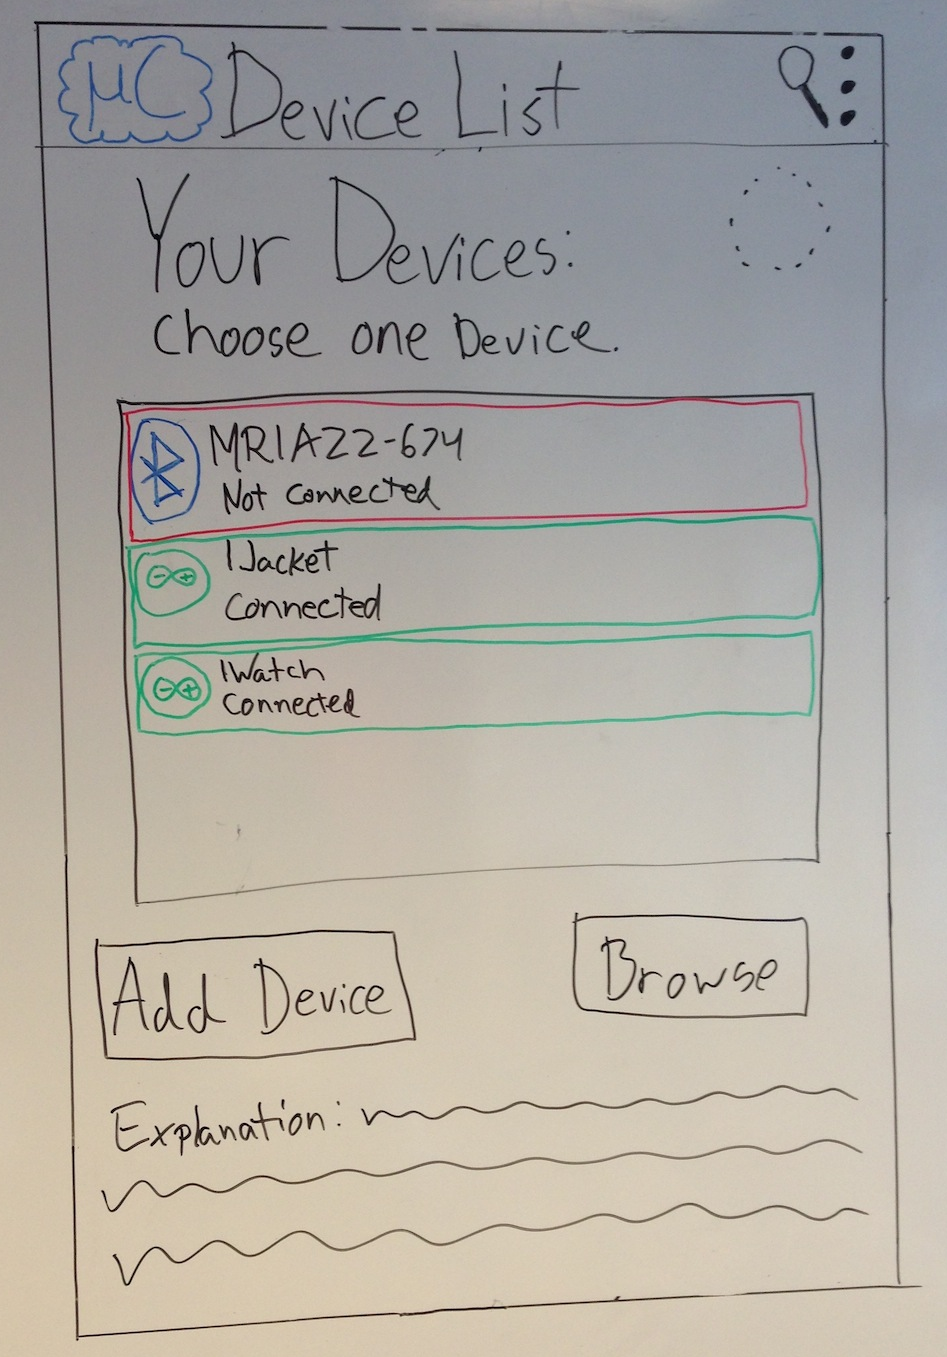
\includegraphics[scale=0.2]{images/Design_guide/Screen1a.png}
	\caption{Screen 1a - Device list}
	\label{fig:screen1a}
\end{figure}


\paragraph{Screen 1b - Add device manually}
Screen that appears after pressing the ``Add device'' button in Screen 1a. It was chosen to remove the ``Bluetooth$\textsuperscript{\textregistered}$ settings'' button, as it proved unnecessary. In the final design, this screen contains only the ``QR code'' button and ``Input serial'' button, with a short description of the functionality of the button between them.

\begin{figure}[H]
	\centering
		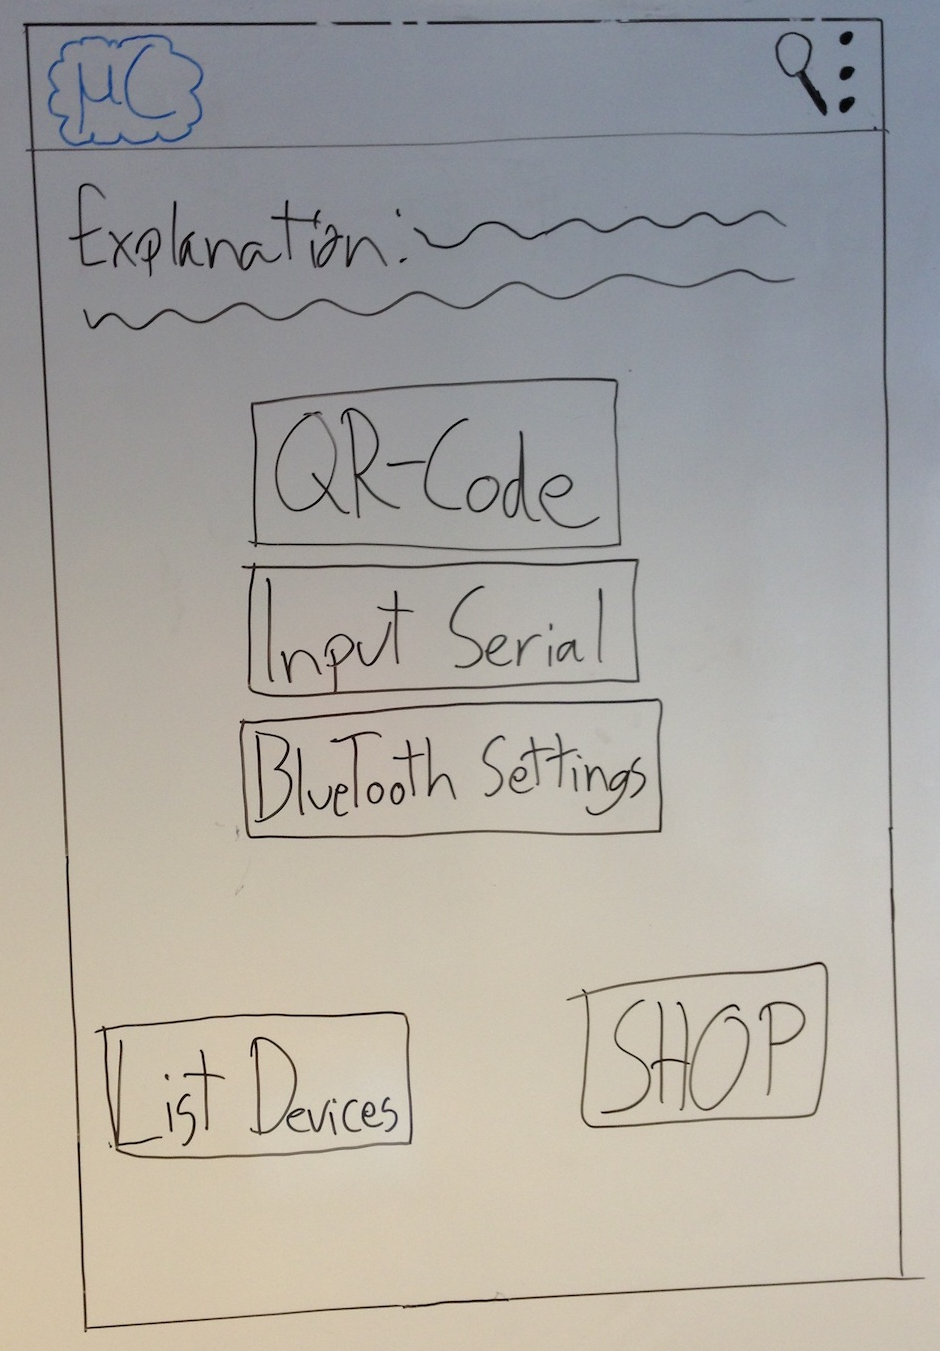
\includegraphics[scale=0.2]{images/Design_guide/Screen1b.png}
	\caption{Screen 1b - Add device manually}
	\label{fig:screen1b}
\end{figure}


\paragraph{Screen 1b-i - Input serial}
%Link to Screen 1b-i
Screen that appears when the ``Input serial'' button is clicked.

\begin{figure}[H]
\centering
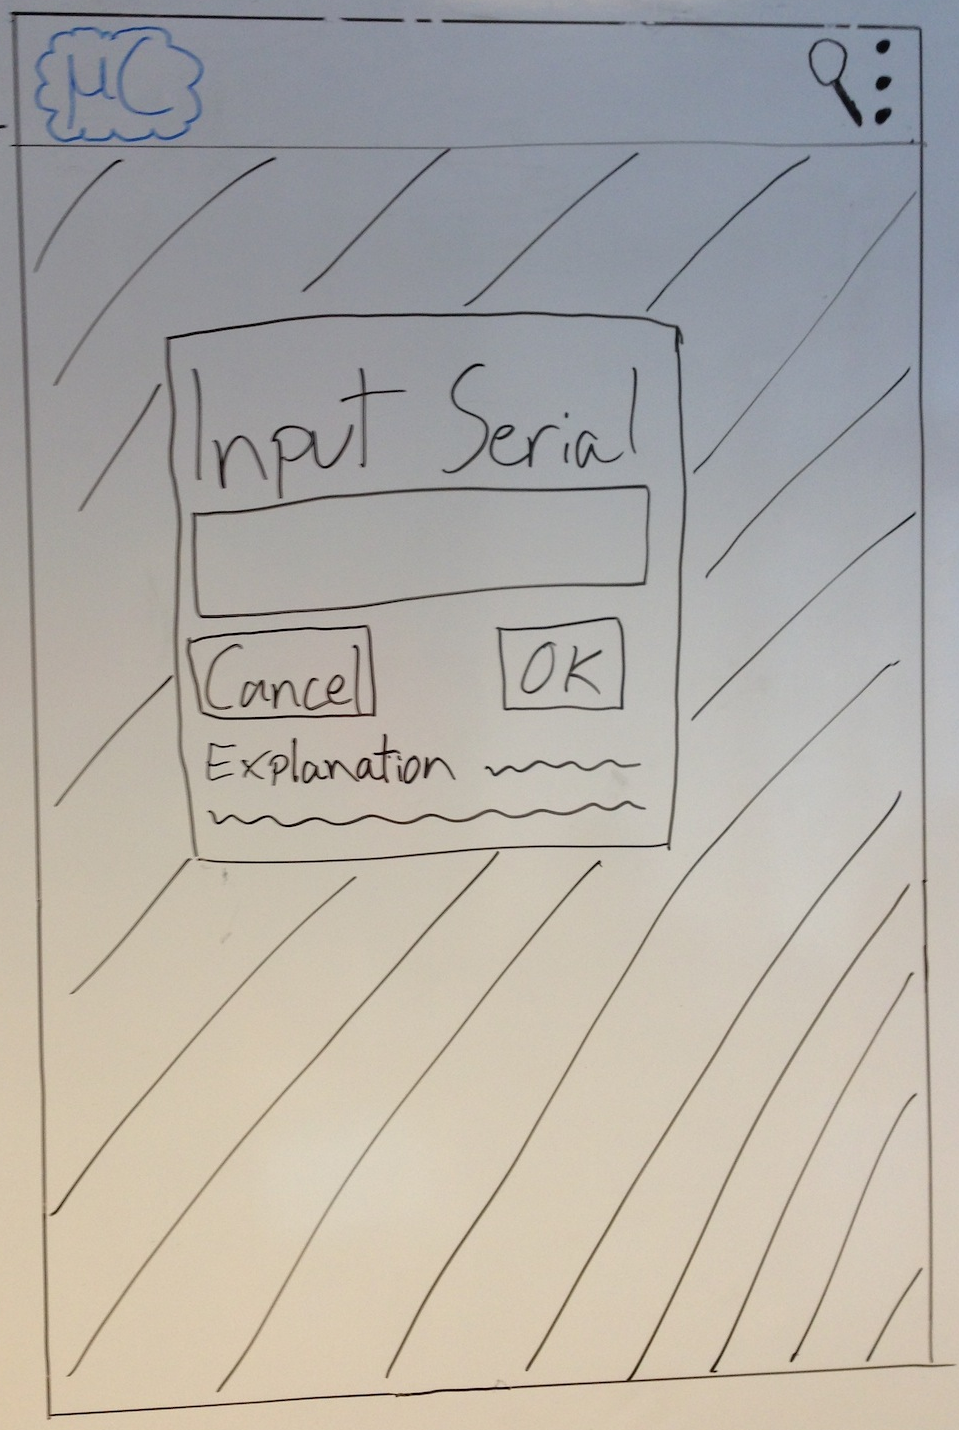
\includegraphics[scale=0.2]{images/Design_guide/Screen1b-i.png}
\caption{Screen 1b-i - Input serial}
\label{fig:screen1bi}
\end{figure}


\paragraph{Screen 2a - Browse shop}
%Link to Screen 2a
Screen for browsing all the applications for Arduino in the shop. More categories have been added. The user can here swipe left/right to sort the available applications in different ways. See next paragraph.

\begin{figure}[H]
\centering
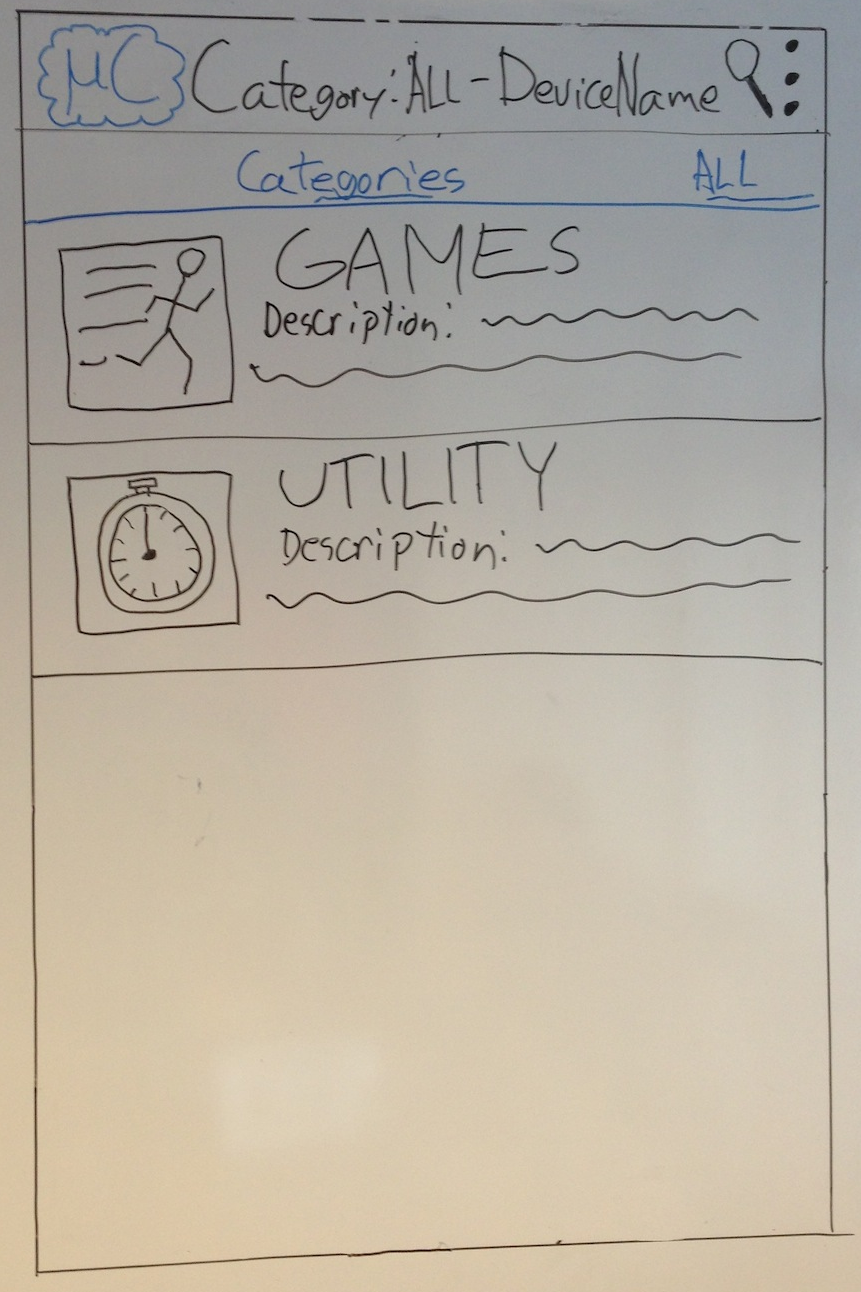
\includegraphics[scale=0.2]{images/Design_guide/Screen2a.png}
\caption{Screen 2a - Browse shop}
\label{fig:screen2a}
\end{figure}


\paragraph{Screen 2b - Browse shop by category}
%Link to Screen 2b
Screen that shows a list of all applications in chosen category. Category ``All'' is chosen.

\begin{figure}[H]
\centering
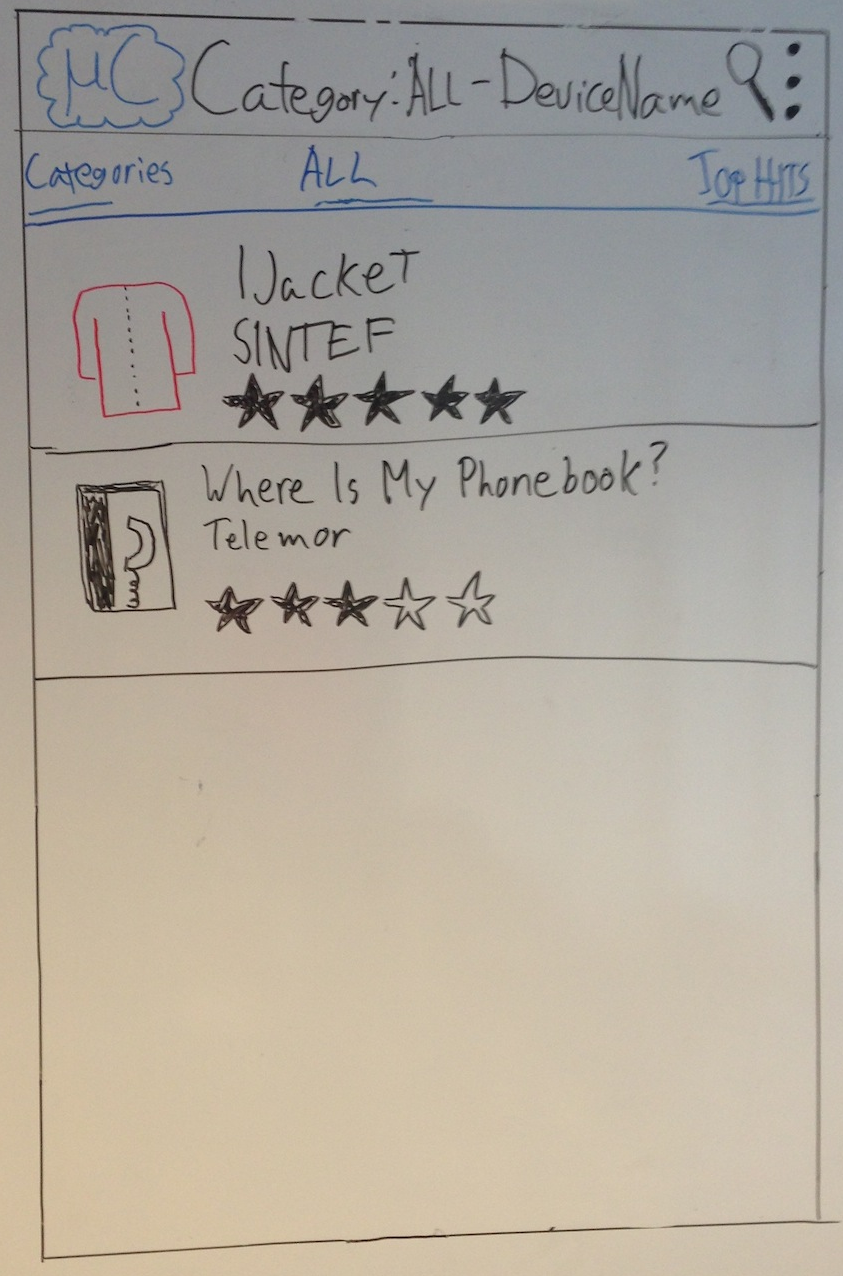
\includegraphics[scale=0.2]{images/Design_guide/Screen2b.png}
\caption{Screen 2b - Browse shop by category}
\label{fig:screen2b}
\end{figure}


\paragraph{Screen 3a - Application view}
%Link to Screen 3a
Screen with overview of an chosen application. Small changes were needed, as the comments field and reviews were given a lower priority at mid-term.

\begin{figure}[H]
\centering
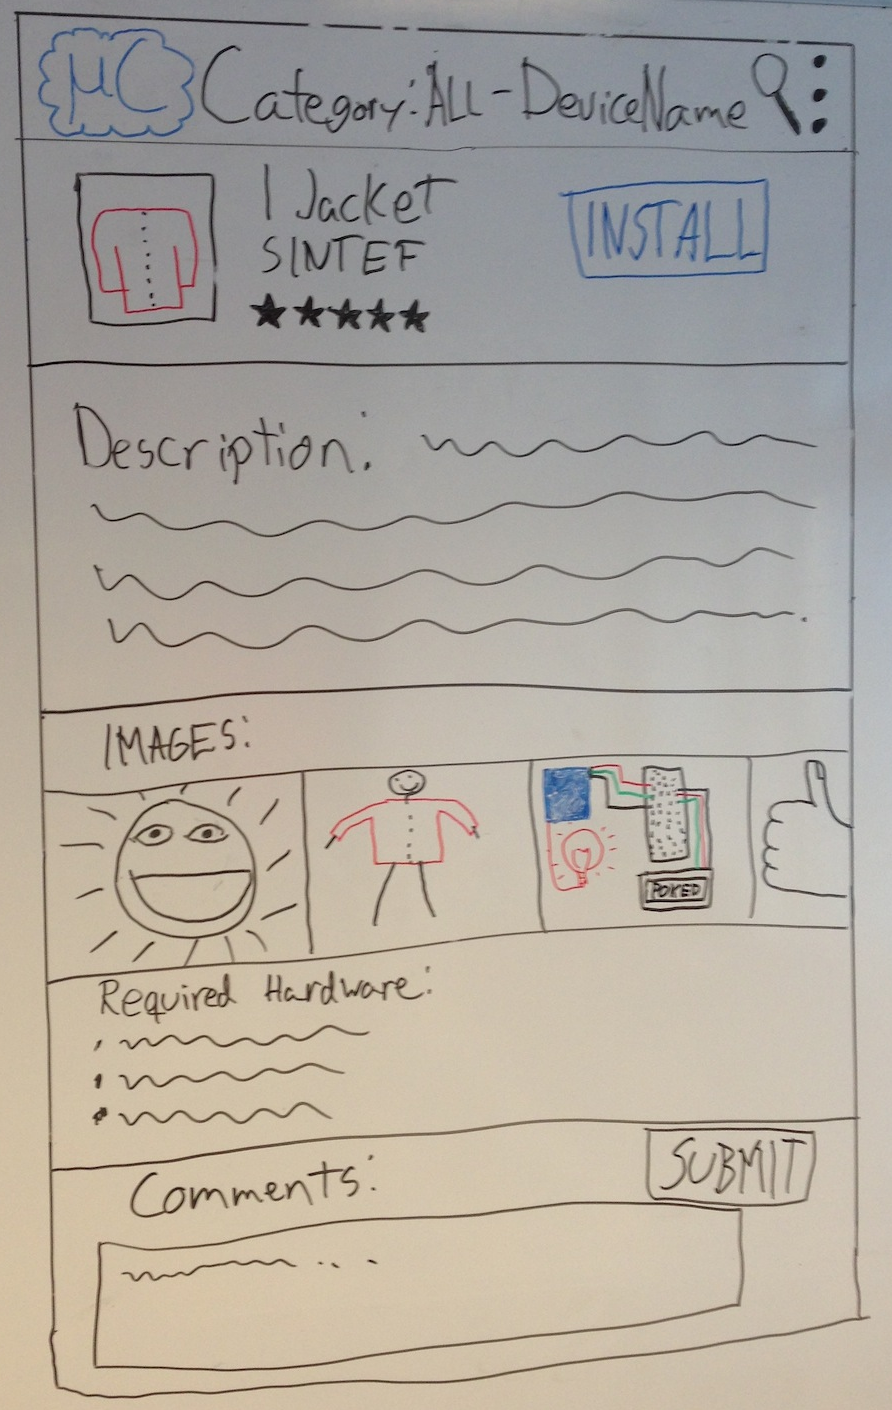
\includegraphics[scale=0.2]{images/Design_guide/Screen3a.png}
\caption{Screen 3a - Application view}
\label{fig:screen3a}
\end{figure}


\paragraph{Screen 3a-i - Installation confirmation}
%Link to Screen 3a-i
Screen that appears when the ``Install'' button in Screen 3a is pressed. Shows the name of the chosen device.

\begin{figure}[H]
\centering
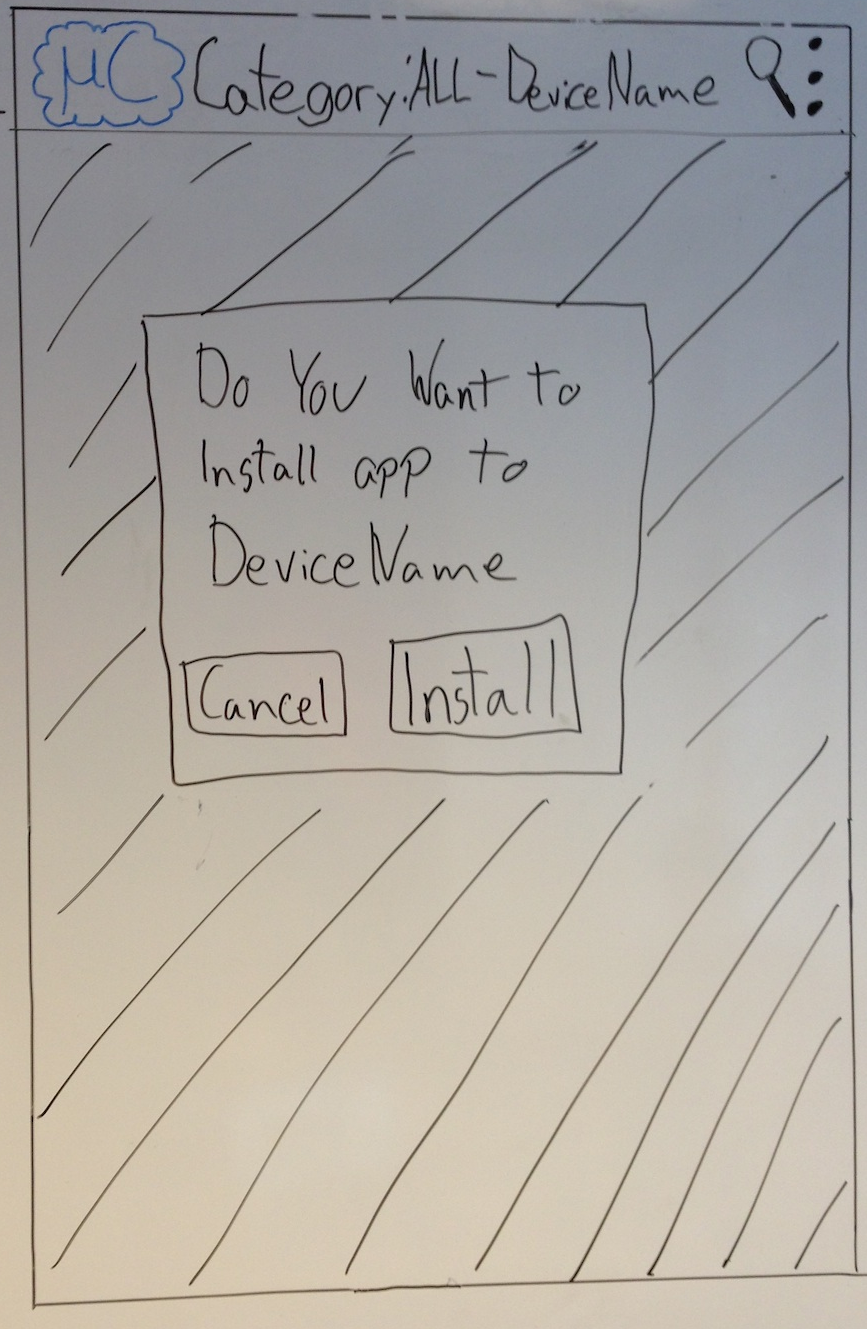
\includegraphics[scale=0.2]{images/Design_guide/Screen3a-i.png}
\caption{Screen 3a-i - Installation confirmation}
\label{fig:screen3ai}
\end{figure}


\paragraph{Screen 3a-ii - Progress of installation}
%Link to Screen 3a-ii
Screen that shows the progress of the installation. The progress bar cannot be dismissed, so the Android application is locked until the installation is complete or has failed.
The user is warned not to move the Android device out of range of the Arduino.

\begin{figure}[H]
\centering
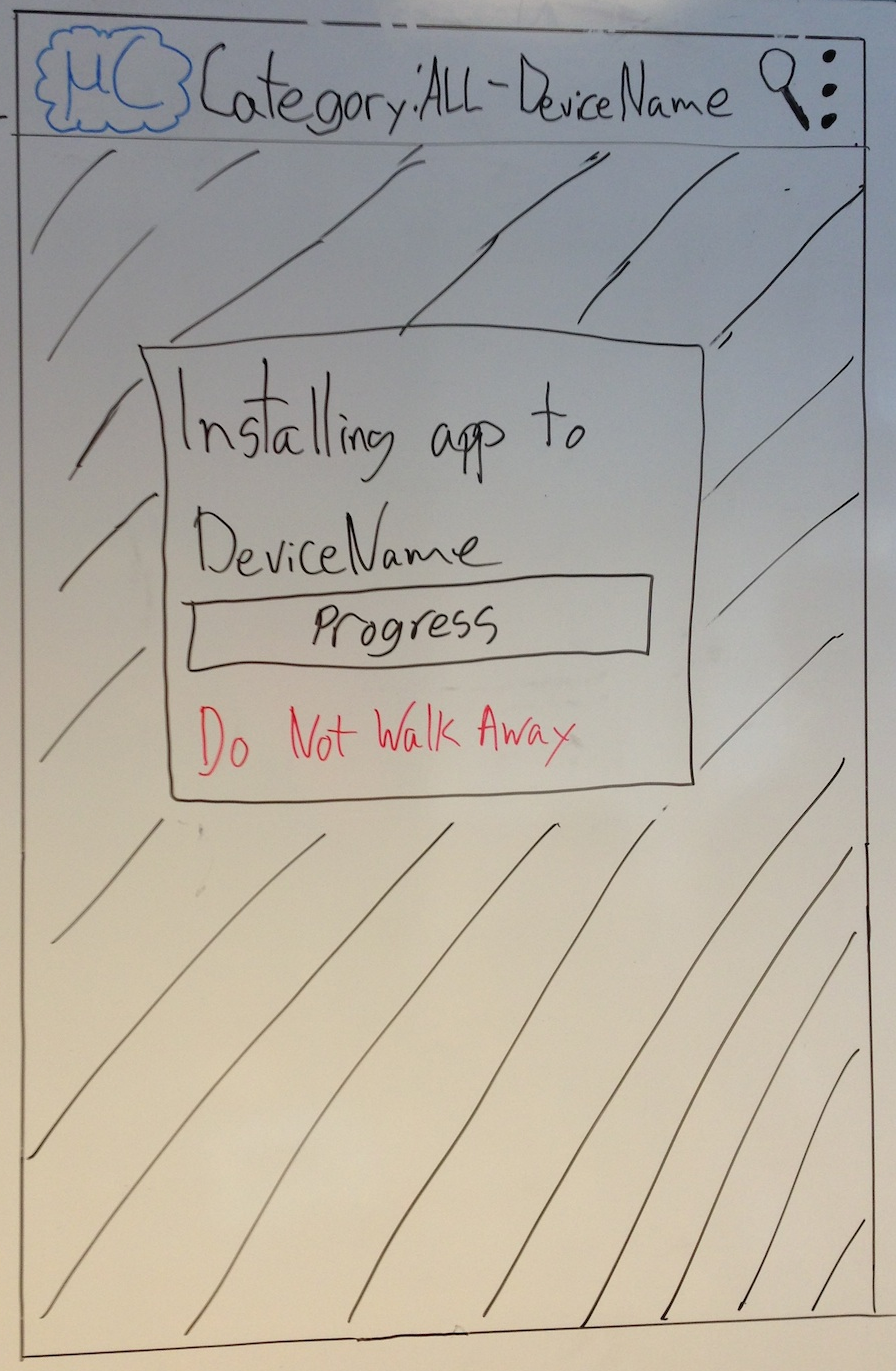
\includegraphics[scale=0.2]{images/Design_guide/Screen3a-ii.png}
\caption{Screen 3a-ii - Progress of installation}
\label{fig:screen3aii}
\end{figure}


\paragraph{Screen Xa - Action overflow}
%Link to Screen Xa
Screen that appears when the ``Action overflow'' button is clicked. This menu is available from all the screen in the application with the exception of the preferences screen.

\begin{figure}[H]
\centering
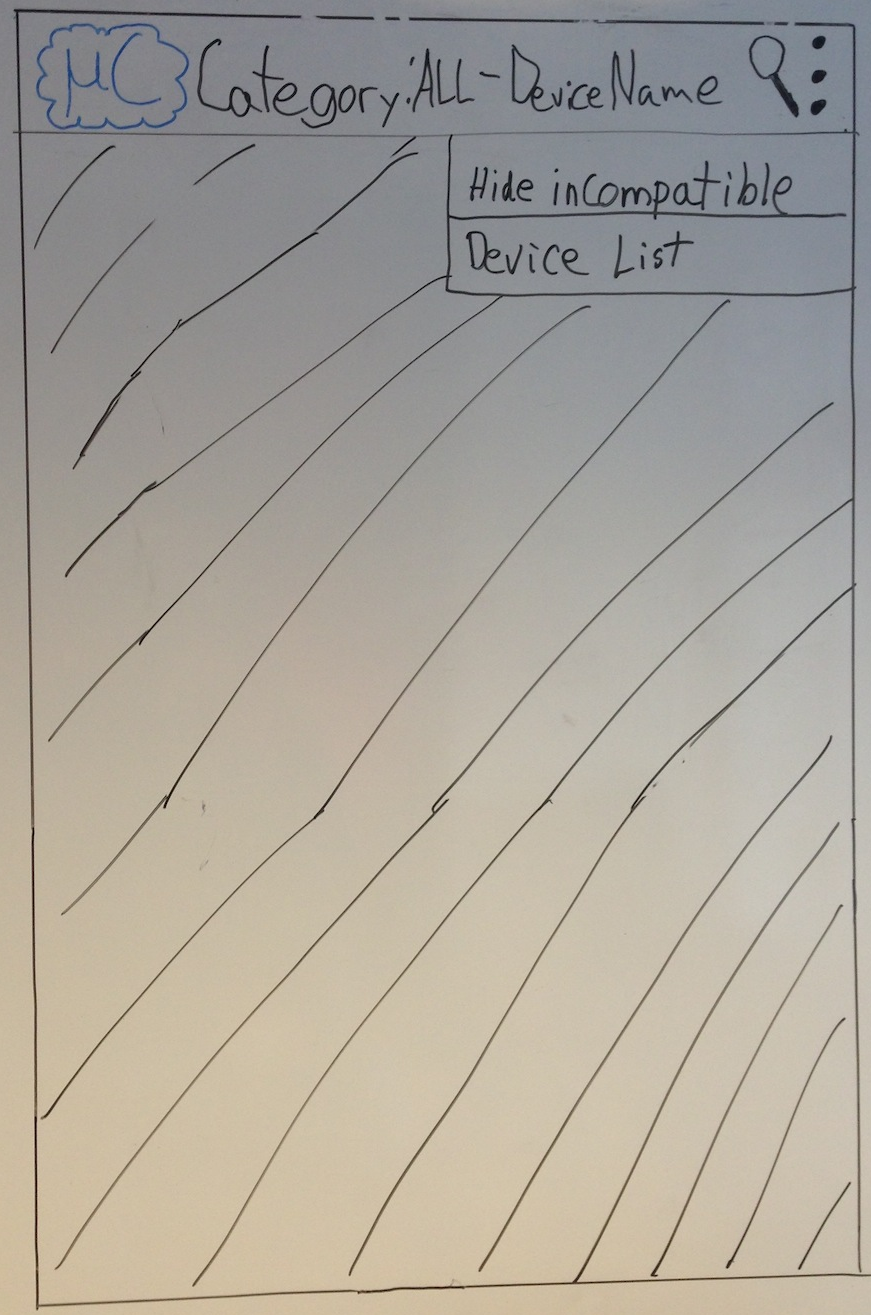
\includegraphics[scale=0.2]{images/Design_guide/ScreenXa.png}
\caption{Screen Xa - Action overflow}
\label{fig:screenXa}
\end{figure}

	\subsection{Decision of design}
	\textbf{Device list}\\
	It should be simple and fit as many devices as possible, even on the smaller cell phones. As shown in Figure~\ref{fig:screen1a} it was decided to use discovered Bluetooth devices as a primary method of connection to an Arduino. That is why the user will meet this screen first. The less frequently used methods for connecting to an Arduino, like QR codes and serial input, were therefore put separately in another screen, as shown in Figure~\ref{fig:screen1b}. \\

	Because of license compatibility issues, it was necessary to use external QR-code readers. To give the user more flexibility, it is therefore possible for the user to select the optimal QR-reader from his application list.\\

	When serial input is clicked, it was decided to open a dialog box for the input string as shown in Figure~\ref{fig:screen1bi}. This is because it clearly gives the user feedback on what is happening and it does not add unnecessary clutter to the GUI.\\

	\textbf{Browse shop}\\
	The category selection as shown in Figure~\ref{fig:screen2a} was done because it groups the applications, and makes it easier for the user to browse for the more specific applications. The swiping was implemented because it easily and quickly selects what to show. This is a fast way to change what to sort the applications by, and is user friendly on a touch screen. ``Top hits'' and ``All'' were chosen because the database is currently small, and it is not necessary with a large amount of ``sort by'' tabs. Other tabs could be easily implemented if need be.\\

	\textbf{Application view}\\
	The application view, as shown in Figure~\ref{fig:screen3a}, should show all the detail and information about an application that is useful and interesting to the user. Rating, description, developer, application name and images were selected for trying to keep a ``standard''. Meaning that both Google Market and AppStore uses these elements and are expected to be familiar for many users.\\

	When the install button is clicked a confirmation box will pop up as shown in Figure~\ref{fig:screen3ai}. This is because the user might have clicked the button on accident or is not informed about what device he/she is connected to. The device name will therefore be shown in this dialog box.\\

	A progress bar will pop up when the user have confirmed the installation. This is because the application should give an indicator on when the application is complete and when its safe to close the application. \\

	\textbf{Action overflow menu}
	When the user clicks on the action overflow menu, he will expect some sort of settings. That is why this menu contains settings. If the user will hide or show incompatible application to his Arduino, this menu will toggle the preference as shown in Figure~\ref{fig:screenXa}.\\

	\textbf{Changes to the design}
	The action overflow menu have two other options: ``Device List'' and ``Populate Database''. This is because this application is only a prototype and it was necessary to hard code Arduino applications into the Android application. The populate database function will therefore feed the local database with some sample applications.\\

	The device list function is there because it should be possible to change device at all times, not only on startup.\\

\section{Database implementation}

	SQLite was used as database language because it is integrated with Android and have much functionality that makes it easy to use in an Android application. Because of changes to priorities the group and the customer got in an agreement to drop the sync adapter, and only use a local database.

	\subsection{Database model}

		In figure~\ref{fig:erdiagram} the database is shown as an ER Diagram. The pictures table was not used because of changes to the teams priorities. Things that had been done before was not important for the customer.

		\begin{figure}[H]
		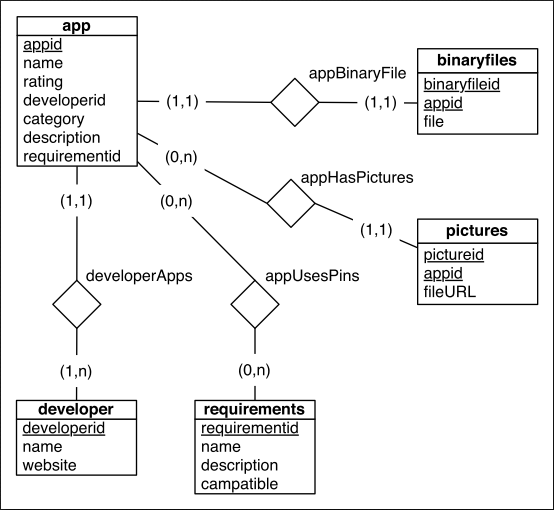
\includegraphics[scale=1]{images/ER_Diagram.png}
		\caption{The ER Diagram describing the setup of the app database.}
		\label{fig:erdiagram}
		\end{figure}

	\subsection{Database details}

		Description and detail about the database tables.

		\subsubsection{Table: app}

			This table contains information about the application.\\

			{\bf \underline{appid}(integer):} auto-increment primary key for applications  \\
			\textbf{name(varchar 160):} name of the application \\
			\textbf{rating(int 10):} rating of the application \\
			\textbf{developerid(int 10):} foreign key to the developer of this application \\
			\textbf{category(varchar 200):} which category this application belongs to \\
			\textbf{description(varchar 200):} description of the application \\
			\textbf{requirementid(int 10):} foreign key to the requirements of this application \\

		\subsubsection{Table: binaryfiles}

			This table contains information about the hex-file (compiled Arduino code). \\
			{\bf \underline{binaryfileid}(integer):} auto-increment primary key for binary files \\
			\textbf{appid(int 10):} foreign key to the application that owns this binary file \\
			\textbf{file(BLOB 1000000):} The binary file in a BLOB \\

			A BLOB is not a datatype and stores data exactly as it was input. This database stores it as a binary array.

		\subsubsection{Table: developer}

			This table contains information about the developer. \\
			{\bf \underline{developerid}(integer):} auto-increment primary key for developers \\
			\textbf{name(varchar 160):} name of the developer \\
			\textbf{website(varchar 200):} website of the developer \\

		\subsubsection{Table: requirements}

			This table contains the requirements for the application. \\
			{\bf \underline{requirementid}(integer):} auto-increment primary key for the requirement \\
			\textbf{name(varchar 160):} name of the requirement \\
			\textbf{description(varchar 200):} description of the requirement \\
			\textbf{compatible(int 10):} integer that is converted to boolean when retrieved from database. \\

			Compatible is an integer of 1 or 0. This indicates if the application referred to is compatible with pagers or not.

		\subsubsection{Table: appusespins}

			This table contains the information about which pins on the Arduino that the application is using. \\
			\textbf{appid(int 10):} foreign key to the application that uses this rule \\
			\textbf{requirementid(int 10):} foreign key to the associated requirement \\

